\documentclass[11pt]{article}

% --- Packages ---
\usepackage[english]{babel}
\usepackage[utf8]{inputenc}
\usepackage[T1]{fontenc}
\usepackage[margin=1in]{geometry}
\usepackage{amsmath, amssymb, amsfonts, amsthm, mathtools}
\usepackage{physics}
\usepackage{graphicx}
\usepackage{booktabs}
\usepackage{array}
\usepackage{enumitem}
\usepackage{fancyhdr}
\usepackage[most]{tcolorbox}
\usepackage[colorlinks=true, allcolors=blue]{hyperref}

\graphicspath{{figures/}}
\setlength{\emergencystretch}{3em}
\numberwithin{equation}{section}

\providecommand{\erf}{\operatorname{erf}}
\providecommand{\erfc}{\operatorname{erfc}}
\newcommand{\lth}{\lambda_{\mathrm{th}}}
\newcommand{\Cq}{C_v^{\mathrm{q}}}
\newcommand{\Ccl}{C_v^{\mathrm{cl}}}
\newcommand{\kB}{k_{B}}

\newtcolorbox{resultbox}[1]{
    colback=lightgray!15, colframe=black, arc=3pt, outer arc=3pt,
    boxrule=0.8pt, left=2mm, right=2mm, top=2mm, bottom=2mm, breakable,
    title={#1}, colbacktitle=gray!20, coltitle=black, fonttitle=\bfseries
}

\pagestyle{fancy}
\fancyhf{}
\lhead{\small 00540367: Research Project 1}
\rhead{\small Technion - IIT}
\lfoot{\small Spring 2026 | Semester 6}
\rfoot{\small Page \thepage}
\renewcommand{\headrulewidth}{0.4pt}
\renewcommand{\footrulewidth}{0.4pt}

\title{Quantum vs.\ Classical Heat Capacity of a Reflectionless\\
P\"oschl--Teller Well in an Infinite Square Well:\\
an Exactly Solvable Case of $\Cq > \Ccl$}
\author{Nadav Jean\\[1mm]
\small Department of Chemical Engineering, Technion -- Israel Institute of Technology}
\date{}

\begin{document}
\maketitle
\thispagestyle{fancy}

\begin{resultbox}{Main results}
For a particle of mass $m$ in the potential
\[
V(x)=-\frac{\hbar^2}{2m}\,\alpha^2\,\frac{2}{\cosh^2(\alpha x)}=-\frac{\hbar^2\alpha^2}{m}\,\frac{1}{\cosh^2(\alpha x)}\quad (|x|<L/2),\qquad V=+\infty\quad(|x|\ge L/2),
\]
i.e.\ the modified P\"oschl--Teller well of Table~I in Ref.~\cite{deffner2014} with $\lambda=2$, inside an infinite square well, and with the thermal wavelength $\lth=\sqrt{2\pi\hbar^2\beta/m}$:
\begin{enumerate}[leftmargin=*,itemsep=2pt]
\item \textbf{Levels (exact, any $L$).} One bound state, $E_b=-\hbar^2\kappa_b^2/2m$ with $\kappa_b=\alpha\tanh(\alpha L/2)\tanh(\kappa_bL/2)$, so $E_b=-(\hbar^2\alpha^2/2m)\,[1+\mathcal O(e^{-\alpha L})]$. Box levels $E_j=\hbar^2k_j^2/2m$, $j=1,2,\dots$, with
$k_jL=j\pi+2\arctan\!\big[k_j/\alpha\tanh(\alpha L/2)\big]$ (Sec.~\ref{sec:levels}).
\item \textbf{Quantum partition function (closed form).} $Z_q=L/\lth-\tfrac12+e^{\beta\hbar^2\alpha^2/2m}\erf\sqrt{\beta\hbar^2\alpha^2/2m}$, up to exponentially small terms. $\Cq=\kB\beta^2\,\mathrm{Var}(E)$ then follows in closed form (Sec.~\ref{sec:quantum}).
\item \textbf{Classical partition function (closed form).} $Z_{\rm cl}=\big[L+I(\beta)\big]/\lth$ with $\alpha I=\sum_{\ell\ge1}(2a)^\ell/[\ell(2\ell-1)!!]=2a\,{}_2F_2(1,1;\tfrac32,2;a)$ and $a=\beta\hbar^2\alpha^2/m$. $\Ccl$ is given in terms of $\erf$ (Sec.~\ref{sec:classical}).
\item \textbf{The $\xi$ formula} is evaluated \emph{exactly} along the ladder $\xi_n=\sqrt{n(n-1)/2}$, where $\xi^2V$ is again reflectionless. Its $n\to\infty$ limit is taken analytically and reproduces $Z_{\rm cl}$; numerically the error falls as $\mathcal O(1/\xi)$ (Sec.~\ref{sec:classical}).
\item \textbf{Anomaly.} $\Cq>\Ccl$ in a window just below the quantum peak. At $\alpha L=1000$ the excess is $+4.80\,\kB$ at $\kB T=0.167\,(\hbar^2\alpha^2/2m)$, where $\Cq=7.45\,\kB$ and $\Ccl=2.65\,\kB$ (Sec.~\ref{sec:results}).
\item \textbf{DVR.} The repo's sinc-DVR reproduces the bound state to $10^{-13}\,(\hbar^2\alpha^2/2m)$, but the box levels only to $\mathcal O(\Delta x)$, because its grid edges act as walls whose position is uncertain by about $\Delta x$. A box (sine) DVR reproduces every level to $10^{-12}\,(\hbar^2\alpha^2/2m)$ (Sec.~\ref{sec:dvr}).
\item \textbf{Scale invariance of the sum.} The well and the box are each scale-invariant in the sense of Ref.~\cite{deffner2014}. Their sum is too when $\alpha\to\alpha/\gamma$ and $L\to\gamma L$ with the same $\gamma$, and only then. Every level then scales as $E_n\to E_n/\gamma^2$, and $C_v(T;\gamma)=C_v(\gamma^2T;1)$ (Sec.~\ref{sec:stroke}).
\end{enumerate}
Every number quoted below is produced by \texttt{verification/pt\_box/pt\_box\_check.py} and recorded in \texttt{RESULTS.md}.
\end{resultbox}

\tableofcontents

% =====================================================================
\section{Motivation and plan}
\label{sec:intro}
The project searches for a potential whose quantum heat capacity $\Cq(T)$ exceeds its classical counterpart $\Ccl(T)$ in some temperature window \cite{gelbwaser2018}. The mechanism identified so far is a single, deep, narrow bound state separated by a gap from a dense, high-entropy set of levels: on heating, the quantum particle leaves a zero-entropy state all at once, producing a sharp Schottky-like peak, while the classical particle in the same well binds more deeply and releases its heat later.

This document formalizes that calculation for a system in which \emph{every} step can be done exactly. The system is a reflectionless P\"oschl--Teller well ($\lambda=2$) inside an infinite square well. It has three properties that make it suitable as a reference case:
\begin{enumerate}[itemsep=1pt]
\item the spectrum is fixed by explicit scalar equations, and the quantum partition function has a closed form (Secs.~\ref{sec:levels}--\ref{sec:quantum});
\item the classical limit can be taken with the project's own $\xi$ formula, exactly and analytically (Sec.~\ref{sec:classical});
\item both components appear in Table~I of Deffner, Jarzynski and del Campo \cite{deffner2014}, and their sum stays scale-invariant, so the system admits homogeneous, scale-invariant strokes (Sec.~\ref{sec:stroke}).
\end{enumerate}
The quantum heat capacity is computed with the variance formula $C_v=\kB\beta^2\mathrm{Var}(E)$ used throughout the project. Sec.~\ref{sec:dvr} uses the exact spectrum as a reference against which the repository's DVR solver is checked.

% =====================================================================
\section{The model}
\label{sec:model}

\subsection{Hamiltonian and potential}
A particle of mass $m$ moves in one dimension with Hamiltonian $H=p^2/2m+V(x)$, where
\begin{equation}
V(x)=\begin{cases}
-\dfrac{\hbar^2}{2m}\,\alpha^2\,\dfrac{\lambda(\lambda-1)}{\cosh^2(\alpha x)}, & |x|<L/2,\\[6pt]
+\infty, & |x|\ge L/2.
\end{cases}
\label{eq:Vgeneral}
\end{equation}
Inside the box this is the modified P\"oschl--Teller well \cite{flugge1971,poschlteller1933}, written exactly as in Table~I of Ref.~\cite{deffner2014} (with $q\to x$). For integer $\lambda$ the well is \emph{reflectionless} \cite{cooper1995}. Throughout we use $\lambda=2$, so $\lambda(\lambda-1)=2$ and
\begin{equation}
V(x)=-\frac{\hbar^2}{2m}\,\alpha^2\,\frac{2}{\cosh^2(\alpha x)}=-\frac{\hbar^2\alpha^2}{m}\,\frac{1}{\cosh^2(\alpha x)}\qquad(|x|<L/2).
\label{eq:V2}
\end{equation}
The well has depth $\hbar^2\alpha^2/m$ (the classical floor is $V_{\min}=-\hbar^2\alpha^2/m$) and width $\sim1/\alpha$, and sits at the centre of a box of length $L$ (Fig.~\ref{fig:potential}). Only $\lambda=2$ represents the physical system. Other integer values of $\lambda$ are needed in Sec.~\ref{sec:classical}, where the $\xi$ formula changes $\lambda$.

\begin{figure}[h]
\centering
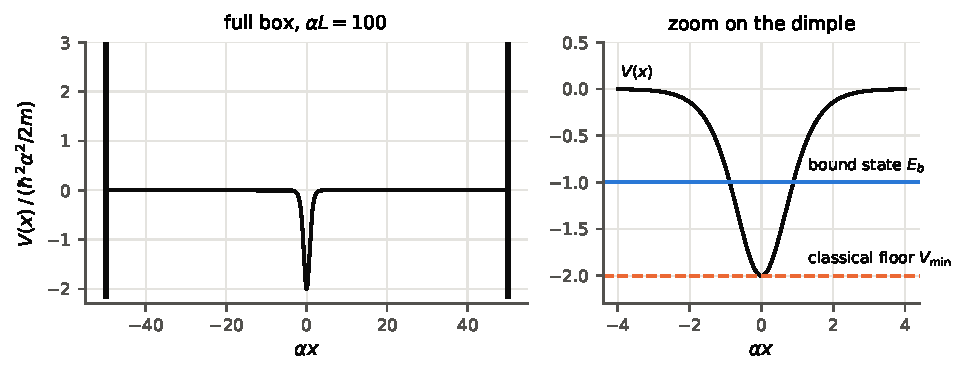
\includegraphics[width=0.95\textwidth]{fig_potential.pdf}
\caption{The potential of Eq.~\eqref{eq:V2} for $\alpha L=100$ (left) and a zoom on the well (right). The single quantum bound state sits at $E_b=-\hbar^2\alpha^2/2m$, halfway up to the continuum threshold from the classical floor $V_{\min}=-\hbar^2\alpha^2/m$.}
\label{fig:potential}
\end{figure}

\subsection{Dimensionless combinations}
All results depend on two dimensionless combinations of the physical constants: the box length in units of the well width, and the temperature in units of the well's energy scale $\hbar^2\alpha^2/2m$,
\begin{equation}
\alpha L\qquad\text{and}\qquad\frac{\kB T}{\hbar^2\alpha^2/2m}=\frac{2m\kB T}{\hbar^2\alpha^2}.
\label{eq:dimless}
\end{equation}
The thermal de Broglie wavelength $\lth=\sqrt{2\pi\hbar^2\beta/m}$ obeys
\begin{equation}
\frac{L}{\lth}=\alpha L\sqrt{\frac{m\kB T}{2\pi\hbar^2\alpha^2}}.
\label{eq:Llth}
\end{equation}
We assume $\alpha L\gg1$, so the well is far from the walls. Corrections from the overlap of the well with the walls are of order $e^{-\alpha L}$ and are negligible for every case studied ($\alpha L\ge30$). Secs.~\ref{sec:quantum} and \ref{sec:classical} show that $\Cq/\kB$ and $\Ccl/\kB$ are functions of the two combinations in Eq.~\eqref{eq:dimless} only. Temperatures are therefore quoted below as $\kB T$ in units of $\hbar^2\alpha^2/2m$.

\subsection{Relation to Table I of Deffner \emph{et al.}}
The well in Eq.~\eqref{eq:Vgeneral} is the ``Modified P\"oschl--Teller well'' row of Table~I in Ref.~\cite{deffner2014}, which the table takes from Fl\"ugge \cite{flugge1971}, with scale-invariant parametrization $\alpha(t)=\alpha(0)/\gamma(t)$ at fixed $\lambda$. The infinite square well is the $b\to\infty$ member of that table's power-law family, with $L(t)=\gamma(t)L(0)$. Each component therefore admits the scale-invariant driving $V(x)\to\gamma^{-2}V(x/\gamma)$ on its own. Section~\ref{sec:stroke} proves that their sum does too, provided both are driven with the same $\gamma$.

% =====================================================================
\section{Energy levels}
\label{sec:levels}

\subsection{Factorization: the well as a partner of the free particle}
Define the superpotential $W(x)=\frac{\hbar\alpha}{\sqrt{2m}}\tanh(\alpha x)$ and the first-order operators
\begin{equation}
A=\frac{\hbar}{\sqrt{2m}}\dv{x}+W(x),\qquad A^\dagger=-\frac{\hbar}{\sqrt{2m}}\dv{x}+W(x).
\end{equation}
Using $W^2=\frac{\hbar^2\alpha^2}{2m}\tanh^2(\alpha x)$, $\frac{\hbar}{\sqrt{2m}}W'=\frac{\hbar^2\alpha^2}{2m}\,\frac{1}{\cosh^2(\alpha x)}$ and $\tanh^2=1-1/\cosh^2$,
\begin{align}
A^\dagger A&=-\frac{\hbar^2}{2m}\dv[2]{x}+\frac{\hbar^2\alpha^2}{2m}\left(\tanh^2(\alpha x)-\frac{1}{\cosh^2(\alpha x)}\right)\nonumber\\
&=-\frac{\hbar^2}{2m}\dv[2]{x}-\frac{\hbar^2\alpha^2}{m}\,\frac{1}{\cosh^2(\alpha x)}+\frac{\hbar^2\alpha^2}{2m}=H_{\rm PT}+\frac{\hbar^2\alpha^2}{2m},\\
AA^\dagger&=-\frac{\hbar^2}{2m}\dv[2]{x}+\frac{\hbar^2\alpha^2}{2m}\left(\tanh^2(\alpha x)+\frac{1}{\cosh^2(\alpha x)}\right)=H_{0}+\frac{\hbar^2\alpha^2}{2m},
\end{align}
where $H_{\rm PT}$ is the $\lambda=2$ well of Eq.~\eqref{eq:V2} and $H_0$ is the free particle; both expressions hold pointwise inside the box. Multiplying $AA^\dagger=H_0+\hbar^2\alpha^2/2m$ on the left by $A^\dagger$ gives the intertwining relation
\begin{equation}
H_{\rm PT}\,A^\dagger=A^\dagger H_0 .
\label{eq:intertwine}
\end{equation}
If $\phi$ solves $H_0\phi=E\phi$, then $A^\dagger\phi$ solves $H_{\rm PT}(A^\dagger\phi)=E\,(A^\dagger\phi)$. Taking $\phi=e^{ikx}$ with $E=\hbar^2k^2/2m$ and dropping a constant factor,
\begin{equation}
\boxed{\;\psi_k(x)=\big(\alpha\tanh(\alpha x)-ik\big)\,e^{ikx},\qquad E=\frac{\hbar^2k^2}{2m}.\;}
\label{eq:jost}
\end{equation}
Equation~\eqref{eq:jost} is a solution of the Schr\"odinger equation \emph{inside the box for every $k$}, real or complex. No boundary condition has been imposed yet. Appendix~\ref{app:check} verifies it by direct differentiation.

\subsection{Solutions of definite parity}
$V$ is even, so the eigenstates have definite parity. The real and imaginary parts of Eq.~\eqref{eq:jost} supply both parities:
\begin{align}
\psi_o(x)&=\mathrm{Re}\,\psi_k=\alpha\tanh(\alpha x)\cos(kx)+k\sin(kx) &&\text{(odd)},\label{eq:psio}\\
\psi_e(x)&=-\mathrm{Im}\,\psi_k=k\cos(kx)-\alpha\tanh(\alpha x)\sin(kx) &&\text{(even)}.\label{eq:psie}
\end{align}
For real $k>0$ neither function vanishes identically.

\subsection{Box levels (\texorpdfstring{$E>0$}{E > 0})}
By parity, $\psi(\pm L/2)=0$ reduces to a single condition at $x=L/2$, where $\alpha\tanh(\alpha x)$ takes the value
\begin{equation}
\alpha\tanh(\alpha L/2)=\alpha\left[1+\mathcal O(e^{-\alpha L})\right].
\end{equation}
Equations~\eqref{eq:psio}--\eqref{eq:psie} then give
\begin{align}
\text{even:}\quad& k\cos(kL/2)=\alpha\tanh(\alpha L/2)\sin(kL/2)\iff \tan(kL/2)=\frac{k}{\alpha\tanh(\alpha L/2)},\\
\text{odd:}\quad& \alpha\tanh(\alpha L/2)\cos(kL/2)+k\sin(kL/2)=0\iff \tan(kL/2)=-\frac{\alpha\tanh(\alpha L/2)}{k} .
\end{align}
With $\varphi(k)=\arctan[k/\alpha\tanh(\alpha L/2)]\in(0,\pi/2)$, the even condition reads $kL/2=\varphi+\ell\pi$. Since $-\alpha\tanh(\alpha L/2)/k=-\cot\varphi=\tan(\varphi+\pi/2)$, the odd condition reads $kL/2=\varphi+\pi/2+\ell\pi$. Both combine into one equation:
\begin{equation}
\boxed{\;k_jL=j\pi+2\arctan\!\left(\frac{k_j}{\alpha\tanh(\alpha L/2)}\right),\qquad E_j=\frac{\hbar^2k_j^2}{2m},\qquad j=1,2,3,\dots\;}
\label{eq:quant}
\end{equation}
Even $j$ gives even states and odd $j$ gives odd states.

\paragraph{Existence and uniqueness.} Let $f(k)=kL-2\arctan[k/\alpha\tanh(\alpha L/2)]$. Then $f(0)=0$ and
\[
f'(k)=L-\frac{2\alpha\tanh(\alpha L/2)}{k^2+\alpha^2\tanh^2(\alpha L/2)}\ge L-\frac{2}{\alpha\tanh(\alpha L/2)}>0
\]
whenever $\alpha L\tanh(\alpha L/2)>2$, i.e.\ $\alpha L\gtrsim2.4$. So $f$ is strictly increasing, and Eq.~\eqref{eq:quant} has exactly one root for each $j\ge1$. Because $0<2\arctan<\pi$, that root lies in the bracket
\begin{equation}
\frac{j\pi}{L}<k_j<\frac{(j+1)\pi}{L}.
\label{eq:bracket}
\end{equation}
The value $j=0$ gives only $k=0$. There $\psi_e\equiv0$, while $\psi_o=\alpha\tanh(\alpha x)$ does not vanish at the wall, so neither is a state.

\subsection{The bound state (\texorpdfstring{$E<0$}{E < 0})}
Set $k=i\kappa$ with $\kappa>0$, so $E=-\hbar^2\kappa^2/2m$. Using $\cos(i\kappa x)=\cosh\kappa x$ and $\sin(i\kappa x)=i\sinh\kappa x$, Eqs.~\eqref{eq:psio}--\eqref{eq:psie} become the real solutions
\begin{equation}
\chi_e(x)=\kappa\cosh(\kappa x)-\alpha\tanh(\alpha x)\sinh(\kappa x),\qquad
\chi_o(x)=\alpha\tanh(\alpha x)\cosh(\kappa x)-\kappa\sinh(\kappa x).
\end{equation}
\begin{itemize}[itemsep=2pt]
\item \textbf{Even:} $\chi_e(L/2)=0\iff$
\begin{equation}
\boxed{\;\kappa_b=\alpha\tanh(\alpha L/2)\tanh(\kappa_bL/2),\qquad E_b=-\frac{\hbar^2\kappa_b^2}{2m}.\;}
\label{eq:bound}
\end{equation}
The function
\[
g(\kappa)=\alpha\tanh(\alpha L/2)\tanh(\kappa L/2)-\kappa
\]
satisfies $g(0)=0$, $g'(0)=\alpha L\tanh(\alpha L/2)/2-1>0$, and is concave, so there is exactly one positive root $\kappa_b<\alpha\tanh(\alpha L/2)<\alpha$. Expanding, $\kappa_b=\alpha(1-4e^{-\alpha L}+\dots)$ and
\begin{equation}
E_b=-\frac{\hbar^2\alpha^2}{2m}\left[1-8e^{-\alpha L}+\dots\right].
\end{equation}
At $\alpha L=60$ the computed value is $E_b/(\hbar^2\alpha^2/2m)=-1.000000000000000$.
\item \textbf{Odd:} $\chi_o(L/2)=0\iff\kappa\tanh(\kappa L/2)=\alpha\tanh(\alpha L/2)$. The left side increases with $\kappa$, so the only root is $\kappa=\alpha$. But $\chi_o\equiv0$ at $\kappa=\alpha$, since $\alpha\tanh(\alpha x)\cosh(\alpha x)=\alpha\sinh(\alpha x)$, so the root is spurious. At $E=-\hbar^2\alpha^2/2m$ the two independent solutions are the even $1/\cosh(\alpha x)$ and the odd $[x/2+\sinh(2\alpha x)/4\alpha]/\cosh(\alpha x)$; the odd one is positive for all $x>0$ and cannot vanish at the wall. Hence there is \emph{no} odd bound state.
\end{itemize}
The spectrum is therefore one bound state, Eq.~\eqref{eq:bound}, plus the box levels of Eq.~\eqref{eq:quant}.

\subsection{Physical reading}
For the empty box, $k_jL=j\pi$. The well shifts every wavenumber up by
\[
\frac{2}{L}\arctan\!\left(\frac{k_j}{\alpha\tanh(\alpha L/2)}\right)\in\left(0,\frac{\pi}{L}\right)
\]
(Table~\ref{tab:levels}), which is the scattering phase shift. As $k\to\infty$ the shift tends to $\pi/L$, so level $j$ of the well approaches level $j+1$ of the empty box. Exactly one state has been removed from the continuum, and it reappears as the bound state (Levinson's theorem).

\begin{table}[h]
\centering
\caption{First box levels at $\alpha L=60$, compared with the empty box $E_j^{(0)}=\hbar^2(j\pi/L)^2/2m$. All energies are in units of $\hbar^2\alpha^2/2m$.}
\label{tab:levels}
\begin{tabular}{cccc}
\toprule
$j$ & $E_j$ (well + box) & $E_j^{(0)}$ (empty box) & shift\\
\midrule
1 & $2.93369203\times10^{-3}$ & $2.74155678\times10^{-3}$ & $+1.921\times10^{-4}$\\
2 & $1.17324157\times10^{-2}$ & $1.09662271\times10^{-2}$ & $+7.662\times10^{-4}$\\
3 & $2.63892433\times10^{-2}$ & $2.46740110\times10^{-2}$ & $+1.715\times10^{-3}$\\
4 & $4.68930453\times10^{-2}$ & $4.38649084\times10^{-2}$ & $+3.028\times10^{-3}$\\
5 & $7.32290633\times10^{-2}$ & $6.85389195\times10^{-2}$ & $+4.690\times10^{-3}$\\
\bottomrule
\end{tabular}
\end{table}

\subsection{Solving the equations}
Equation~\eqref{eq:quant} is solved by the fixed-point iteration
\begin{equation}
k\;\leftarrow\;\frac{j\pi+2\arctan[k/\alpha\tanh(\alpha L/2)]}{L},\qquad k^{(0)}=\frac{j\pi}{L},
\end{equation}
which contracts with factor $|\partial k_{\rm new}/\partial k|\le2/[\alpha L\tanh(\alpha L/2)]$. That is $0.033$ at $\alpha L=60$, so a few iterations reach machine precision. All $j$ are iterated at once as a vector. Equation~\eqref{eq:bound} is iterated the same way, starting from $\kappa=\alpha$. For 3000 levels at $\alpha L=60$, the residual $\max_j|k_jL-j\pi-2\arctan[k_j/\alpha\tanh(\alpha L/2)]|$ is $1.4\times10^{-12}$.

\subsection{General integer \texorpdfstring{$\lambda$}{lambda}}
\label{sec:generallambda}
The $\xi$ formula of Sec.~\ref{sec:classical} needs Eq.~\eqref{eq:Vgeneral} for integer $\lambda>2$. With $W_\nu=\frac{\hbar\alpha}{\sqrt{2m}}(\nu-1)\tanh(\alpha x)$, the same algebra gives $A_\nu^\dagger A_\nu=H_\nu+(\nu-1)^2\hbar^2\alpha^2/2m$ and $A_\nu A_\nu^\dagger=H_{\nu-1}+(\nu-1)^2\hbar^2\alpha^2/2m$, where $H_\nu$ is the well with parameter $\nu$. Hence $H_\nu A_\nu^\dagger=A_\nu^\dagger H_{\nu-1}$, and iterating from the free particle ($\nu=1$),
\begin{equation}
\psi_k^{(\lambda)}=A_\lambda^\dagger A_{\lambda-1}^\dagger\cdots A_2^\dagger\,e^{ikx},\qquad A_\nu^\dagger\propto-\dv{x}+(\nu-1)\alpha\tanh(\alpha x).
\end{equation}
For $\alpha x\gg1$, $\tanh\to1$ up to $\mathcal O(e^{-2\alpha x})$, so $\psi_k^{(\lambda)}\to\prod_{p=1}^{\lambda-1}(p\alpha-ik)\,e^{ikx}=|c|\,e^{i[kx-\varphi_\lambda(k)]}$ with $\varphi_\lambda(k)=\sum_{p=1}^{\lambda-1}\arctan[k/(p\alpha)]$. Since $\psi_k^{(\lambda)}(-x)=(-1)^{\lambda-1}[\psi_k^{(\lambda)}(x)]^*$ for real $k$, the real and imaginary parts again have definite parity. The wall condition then gives
\begin{equation}
k_jL=j\pi+2\sum_{p=1}^{\lambda-1}\arctan\!\left(\frac{k_j}{p\alpha}\right)+\mathcal O(e^{-\alpha L}),\qquad
E_p^{\rm bound}=-p^2\,\frac{\hbar^2\alpha^2}{2m},\quad p=1,\dots,\lambda-1.
\label{eq:quantgen}
\end{equation}
The bound-state energies are the P\"oschl--Teller values \cite{poschlteller1933,cooper1995}. For $\lambda=2$ this reduces to Eqs.~\eqref{eq:quant}--\eqref{eq:bound} with $\alpha\tanh(\alpha L/2)\to\alpha$. Table~\ref{tab:generallambda} confirms Eq.~\eqref{eq:quantgen} against a box DVR.

\begin{table}[h]
\centering
\caption{Equation~\eqref{eq:quantgen} against the box sine-DVR of Appendix~\ref{app:sinedvr}, for $\alpha L=40$ and the lowest 80 levels. Energies are in units of $\hbar^2\alpha^2/2m$.}
\label{tab:generallambda}
\begin{tabular}{ccc}
\toprule
$\lambda$ & bound states $E$ & $\max|E^{\rm DVR}-E^{\rm Eq.~\eqref{eq:quantgen}}|$\\
\midrule
2 & $-1$ & $2.4\times10^{-12}$\\
3 & $-4,\,-1$ & $2.4\times10^{-12}$\\
4 & $-9,\,-4,\,-1$ & $2.9\times10^{-12}$\\
6 & $-25,\,-16,\,-9,\,-4,\,-1$ & $2.8\times10^{-12}$\\
\bottomrule
\end{tabular}
\end{table}

% =====================================================================
\section{Quantum heat capacity}
\label{sec:quantum}

\subsection{The variance formula}
For a discrete spectrum $\{E_n\}$ the canonical partition function is $Z=\sum_ne^{-\beta E_n}$. The moments are $\expval{E}=-\partial_\beta\ln Z=Z^{-1}\sum_nE_ne^{-\beta E_n}$ and $\expval{E^2}=Z^{-1}\partial_\beta^2Z=Z^{-1}\sum_nE_n^2e^{-\beta E_n}$. Since $\partial_T=-\kB\beta^2\partial_\beta$,
\begin{equation}
C_v=\pdv{\expval{E}}{T}=\kB\beta^2\left(\expval{E^2}-\expval{E}^2\right)=\kB\beta^2\,\mathrm{Var}(E),
\label{eq:var}
\end{equation}
as derived in the project summaries. Here the spectrum is $\{E_b\}\cup\{E_j\}_{j\ge1}$:
\begin{equation}
Z_q(\beta)=e^{-\beta E_b}+\sum_{j=1}^{\infty}e^{-\beta E_j}.
\label{eq:Zq}
\end{equation}

\subsection{Direct evaluation}
The sums are truncated at $j_{\max}$ with $\beta E_{j_{\max}}\ge45$ at the hottest temperature considered. Since $E_j\approx\hbar^2(j\pi/L)^2/2m$, this means $j_{\max}\approx(L/\pi)\sqrt{90\,m\kB T_{\max}/\hbar^2}$, which is 4795 levels for $\alpha L=1000$ and $\kB T_{\max}=5\,(\hbar^2\alpha^2/2m)$. The neglected Boltzmann weight is below $e^{-45}$ relative to the retained weight. Each weight is computed as $e^{-\beta(E_n-E_b)}$, with the common factor cancelling in the ratios. This is the same exponent shift the pipeline uses, and it prevents overflow. Then
\begin{equation}
\frac{\Cq}{\kB}=\beta^2\left[\frac{\sum_nE_n^2w_n}{\sum_nw_n}-\left(\frac{\sum_nE_nw_n}{\sum_nw_n}\right)^2\right],\qquad w_n=e^{-\beta(E_n-E_b)}.
\label{eq:Cqsum}
\end{equation}

\subsection{Closed form of \texorpdfstring{$Z_q$}{Zq}}
\label{sec:Zclosed}
The level sum in Eq.~\eqref{eq:Zq} can be done analytically. Let $j(k)=\{kL-2\arctan[k/\alpha\tanh(\alpha L/2)]\}/\pi$ be the counting function implied by Eq.~\eqref{eq:quant}, let $k(j)$ be its inverse, and let $F(j)=\exp[-\beta\hbar^2k(j)^2/2m]$, so $\sum_{j\ge1}e^{-\beta E_j}=\sum_{j\ge1}F(j)$.

Since $\arctan$ is odd, $j(k)$ and $k(j)$ are odd, and $F$ is even in $j$ with $F(0)=1$. For an even function, Poisson summation gives
\begin{equation}
\sum_{j=1}^{\infty}F(j)=\int_0^\infty F(j)\,\dd j-\frac12+R,\qquad R=\sum_{\ell\ge1}\hat F(\ell),\quad\hat F(\ell)=\int_{-\infty}^{\infty}F(y)e^{-2\pi i\ell y}\dd y .
\label{eq:poisson}
\end{equation}
The remainder $R$ is exponentially small. For the empty box it is $R=(2L/\lth)\sum_{\ell\ge1}e^{-4\pi\ell^2(L/\lth)^2}$, and the well adds further terms that are exponentially small in $\alpha L$. For every case in this document $R$ is below double precision (Table~\ref{tab:Zcheck}).

Changing variables $j\to k$, with
\[
\frac{\dd j}{\dd k}=\frac1\pi\left[L-\frac{2\alpha\tanh(\alpha L/2)}{k^2+\alpha^2\tanh^2(\alpha L/2)}\right],
\]
and writing $b=\beta\hbar^2/2m$,
\begin{align}
\int_0^\infty F\,\dd j&=\frac{L}{\pi}\int_0^\infty e^{-bk^2}\dd k-\frac{2\alpha\tanh(\alpha L/2)}{\pi}\int_0^\infty\frac{e^{-bk^2}}{k^2+\alpha^2\tanh^2(\alpha L/2)}\dd k\nonumber\\
&=\frac{L}{\lth}-e^{b\alpha^2\tanh^2(\alpha L/2)}\erfc\!\big(\alpha\tanh(\alpha L/2)\sqrt b\big).
\end{align}
Here $\frac{L}{\pi}\cdot\frac12\sqrt{\pi/b}=L/\sqrt{4\pi b}=L/\lth$, and the second integral is evaluated in Appendix~\ref{app:gaussint} with $c=\alpha\tanh(\alpha L/2)$. Adding the bound state $e^{-\beta E_b}=e^{\beta\hbar^2\kappa_b^2/2m}$,
\begin{equation}
Z_q=\frac{L}{\lth}-\frac12+e^{\beta\hbar^2\kappa_b^2/2m}-e^{\beta\frac{\hbar^2\alpha^2}{2m}\tanh^2(\alpha L/2)}\erfc\!\left(\sqrt{\beta\frac{\hbar^2\alpha^2}{2m}}\tanh(\alpha L/2)\right)+R .
\end{equation}
Since $\kappa_b$ and $\alpha\tanh(\alpha L/2)$ both equal $\alpha\,[1+\mathcal O(e^{-\alpha L})]$, this becomes
\begin{equation}
\boxed{\;Z_q(\beta)=\frac{L}{\lth}-\frac12+\exp\!\left(\beta\frac{\hbar^2\alpha^2}{2m}\right)\erf\!\sqrt{\beta\frac{\hbar^2\alpha^2}{2m}}\,.\;}
\label{eq:Zqclosed}
\end{equation}
The three terms have direct meanings. $L/\lth-\tfrac12$ is the empty box, with $-\tfrac12$ the wall (Dirichlet) correction. $e^{\beta\hbar^2\alpha^2/2m}$ is the bound state. The term $-e^{\beta\hbar^2\alpha^2/2m}\erfc\sqrt{\beta\hbar^2\alpha^2/2m}$ is the continuum state lost to the bound state, spread over energy by the phase shift. The same steps applied to Eq.~\eqref{eq:quantgen} give, for any integer $\lambda$,
\begin{equation}
Z_q^{(\lambda)}(\beta)=\frac{L}{\lth}-\frac12+\sum_{p=1}^{\lambda-1}\exp\!\left(\beta p^2\frac{\hbar^2\alpha^2}{2m}\right)\erf\!\left(p\sqrt{\beta\frac{\hbar^2\alpha^2}{2m}}\right).
\label{eq:Zqgen}
\end{equation}
This is equivalent to the Beth--Uhlenbeck form of the partition function \cite{bethuhlenbeck1937} with the reflectionless phase shifts.

\subsection{Closed-form \texorpdfstring{$\Cq$}{Cq}}
Write Eq.~\eqref{eq:Zqclosed} as $Z_q=A\beta^{-1/2}-\tfrac12+G(\beta)$, with $A=L\sqrt{m/2\pi\hbar^2}$ and
\[
G(\beta)=\exp\!\left(\beta\frac{\hbar^2\alpha^2}{2m}\right)\erf\sqrt{\beta\frac{\hbar^2\alpha^2}{2m}} .
\]
Since
\[
\dv{\beta}\erf\sqrt{\beta\frac{\hbar^2\alpha^2}{2m}}=e^{-\beta\hbar^2\alpha^2/2m}\,\frac{\hbar\alpha}{\sqrt{2\pi m\beta}},
\]
\begin{equation}
G'=\frac{\hbar^2\alpha^2}{2m}\,G+\frac{\hbar\alpha}{\sqrt{2\pi m\beta}},\qquad
G''=\frac{\hbar^2\alpha^2}{2m}\,G'-\frac{\hbar\alpha}{2\sqrt{2\pi m}}\,\beta^{-3/2},
\end{equation}
\begin{equation}
Z_q'=-\frac A2\beta^{-3/2}+G',\qquad Z_q''=\frac{3A}{4}\beta^{-5/2}+G''.
\end{equation}
Since $\expval{E}=-Z_q'/Z_q$ and $\expval{E^2}=Z_q''/Z_q$, Eq.~\eqref{eq:var} becomes
\begin{equation}
\boxed{\;\frac{\Cq}{\kB}=\beta^2\left[\frac{Z_q''}{Z_q}-\left(\frac{Z_q'}{Z_q}\right)^2\right].\;}
\label{eq:Cqclosed}
\end{equation}
Since $\beta\hbar^2\alpha^2/2m$ and $A\beta^{-1/2}=L/\lth$ (Eq.~\eqref{eq:Llth}) are functions of $\alpha L$ and $2m\kB T/\hbar^2\alpha^2$ only, so is the right side. For integer $\lambda$, $G$ becomes $\sum_pG_p$ with $\hbar^2\alpha^2/2m\to p^2\hbar^2\alpha^2/2m$ in each $G_p$.

\paragraph{Limits.}
\begin{itemize}[itemsep=2pt]
\item As $T\to0$, $Z_q\to e^{\beta\hbar^2\alpha^2/2m}$ and $\Cq\to0$ exponentially, because of the gap $\hbar^2\alpha^2/2m$ between the bound state and the continuum.
\item As $T\to\infty$, $G$ and the classical well term agree at leading order (Sec.~\ref{sec:walls}), so only the wall term $-\tfrac12$ distinguishes $Z_q$ from $Z_{\rm cl}$. It gives $\Cq\to\kB[\tfrac12+\lth/(8L)]$.
\end{itemize}

\subsection{Consistency check}
Table~\ref{tab:Zcheck} compares the direct sum over the exact levels, Eqs.~\eqref{eq:Zq} and \eqref{eq:Cqsum}, with the closed forms of Eqs.~\eqref{eq:Zqclosed} and \eqref{eq:Cqclosed}. They agree to machine precision for all $\kB T\in[0.02,5]\,(\hbar^2\alpha^2/2m)$.

\begin{table}[h]
\centering
\caption{Level sum vs.\ closed form, over 500 temperatures $\kB T\in[0.02,5]\,(\hbar^2\alpha^2/2m)$.}
\label{tab:Zcheck}
\begin{tabular}{cccc}
\toprule
$\alpha L$ & max rel.\ diff.\ $\ln Z_q$ & max $|\Delta\Cq|/\kB$ & levels used\\
\midrule
60 & $2.2\times10^{-16}$ & $7.3\times10^{-13}$ & 307\\
100 & $2.2\times10^{-16}$ & $4.9\times10^{-13}$ & 498\\
1000 & $2.2\times10^{-16}$ & $1.1\times10^{-12}$ & 4795\\
\bottomrule
\end{tabular}
\end{table}

% =====================================================================
\section{Classical heat capacity}
\label{sec:classical}

\subsection{The \texorpdfstring{$\xi$}{xi} formula}
Following \cite{gelbwaser2018} and the project summaries, scaling the potential by $\xi^2$ is equivalent to scaling $\hbar$:
\begin{equation}
\frac{E_n\!\left(\hbar,\ \xi^2V\right)}{\xi^2}=E_n\!\left(\frac{\hbar}{\xi},\ V\right).
\label{eq:xiid}
\end{equation}
Scaling $V\to\xi^2V$ and $T\to\xi^2T$ in Eq.~\eqref{eq:var} therefore gives
\begin{equation}
C_v^{(\xi)}(T)=\kB\left(\frac{\beta}{\xi^2}\right)^2\mathrm{Var}_{\xi^2V}(E)\Big|_{w_n=e^{-\beta E_n/\xi^2}}=\kB\beta^2\,\mathrm{Var}_{\hbar/\xi}(E),\qquad
\Ccl(T)=\lim_{\xi\to\infty}C_v^{(\xi)}(T).
\label{eq:xiformula}
\end{equation}
As in the project's box derivation, the walls are unchanged by the scaling ($\xi^2\cdot\infty=\infty$).

\subsection{Why a generic \texorpdfstring{$\xi$}{xi}-scan is problematic here}
In the language of Eq.~\eqref{eq:xiid}, the well $\xi^2V_{\rm PT}$ with $\hbar$ is the same as $V_{\rm PT}$ with $\hbar_\xi=\hbar/\xi$. Since
$\xi^2\frac{\hbar^2\alpha^2}{2m}\lambda(\lambda-1)=\frac{\hbar_\xi^2\alpha^2}{2m}\lambda_\xi(\lambda_\xi-1)$, the scaled well has
\begin{equation}
\lambda_\xi(\lambda_\xi-1)=\xi^2\lambda(\lambda-1)=2\xi^2\quad\Longrightarrow\quad\lambda_\xi=\tfrac12+\sqrt{\tfrac14+2\xi^2}.
\label{eq:lamxi}
\end{equation}
For a generic $\xi$, $\lambda_\xi$ is not an integer. The scaled well is then no longer reflectionless, and the closed forms of Secs.~\ref{sec:levels}--\ref{sec:quantum} do not apply. A generic $\xi$-scan would need a fresh numerical box spectrum at every $\xi$, with about $\xi$ times more levels ($N\approx\xi\,(L/\pi)\sqrt{90\,m\kB T/\hbar^2}$), and Sec.~\ref{sec:dvr} shows that the repo's DVR does not represent the walls exactly.

\subsection{The integer ladder: an exact \texorpdfstring{$\xi$}{xi}-scan}
Equation~\eqref{eq:lamxi} gives an integer $\lambda_\xi=n$ exactly when
\begin{equation}
\xi=\xi_n\equiv\sqrt{\frac{n(n-1)}{2}},\qquad n=2,3,4,\dots\qquad(\xi_2=1,\ \xi_3=\sqrt3,\ \xi_4=\sqrt6,\ \dots\to\infty).
\label{eq:ladder}
\end{equation}
$\xi_2=1$ is the physical system. Taking the limit in Eq.~\eqref{eq:xiformula} along this sequence is enough, provided the limit exists. Here it does, and the result is obtained in closed form below. At $\xi=\xi_n$ all of Secs.~\ref{sec:generallambda} and \ref{sec:Zclosed} apply with $\hbar\to\hbar/\xi_n$, i.e.\ $\hbar^2\alpha^2/2m\to\hbar^2\alpha^2/(2m\xi_n^2)$ and $\lth\to\lth/\xi_n$. Equation~\eqref{eq:Zqgen} with $\lambda=n$ then gives
\begin{equation}
\boxed{\;Z^{(n)}(\beta)=\xi_n\frac{L}{\lth}-\frac12+\sum_{p=1}^{n-1}\exp\!\left(\beta\frac{\hbar^2\alpha^2}{2m}\frac{p^2}{\xi_n^2}\right)\erf\!\left(\frac{p}{\xi_n}\sqrt{\beta\frac{\hbar^2\alpha^2}{2m}}\right),\;}
\label{eq:Zn}
\end{equation}
and $C_v^{(\xi_n)}$ follows exactly from Eq.~\eqref{eq:Cqclosed}. The scaled well has $n-1$ bound states, at $-p^2\hbar^2\alpha^2/(2m\xi_n^2)$. The deepest is $-(n-1)^2\hbar^2\alpha^2/(2m\xi_n^2)=-(\hbar^2\alpha^2/m)(n-1)/n\to-\hbar^2\alpha^2/m=V_{\min}$. As $\xi$ grows, the bound states fill the classical range of bound energies $[-\hbar^2\alpha^2/m,0)$.

\subsection{The limit \texorpdfstring{$n\to\infty$}{n to infinity}}
Let $h_n=1/\sqrt{n(n-1)}=1/(\sqrt2\xi_n)$, $s_p=ph_n$ and $a\equiv\beta\hbar^2\alpha^2/m$ ($\beta$ times the well depth). Then $\beta\frac{\hbar^2\alpha^2}{2m}\frac{p^2}{\xi_n^2}=as_p^2$ and $\frac{p}{\xi_n}\sqrt{\beta\hbar^2\alpha^2/2m}=s_p\sqrt a$, so the sum in Eq.~\eqref{eq:Zn} is $\sum_{p=1}^{n-1}F(s_p)$ with
\begin{equation}
F(s)=e^{as^2}\erf\!\left(s\sqrt a\right),\qquad F(0)=0,\qquad s_{n-1}=\sqrt{(n-1)/n}\to1 .
\end{equation}
This is a Riemann sum with spacing $h_n$, so $\sum_{p=1}^{n-1}F(ph_n)=h_n^{-1}\int_0^1F(s)\,\dd s+\mathcal O(1)$, and
\begin{equation}
Z^{(n)}(\beta)=\xi_n\,\mathcal Z(\beta)+\mathcal O(1),\qquad
\mathcal Z(\beta)\equiv\frac{L}{\lth}+\sqrt2\int_0^1e^{as^2}\erf\!\left(s\sqrt a\right)\dd s .
\label{eq:Zlimit}
\end{equation}
Hence $\ln Z^{(n)}=\ln\xi_n+\ln\mathcal Z+\mathcal O(1/\xi_n)$. The constant $\ln\xi_n$ does not depend on $\beta$ and drops out of $C_v=\kB\beta^2\partial_\beta^2\ln Z$, so
\begin{equation}
\Ccl=\kB\beta^2\,\partial_\beta^2\ln\mathcal Z(\beta),\qquad C_v^{(\xi_n)}-\Ccl=\mathcal O(1/\xi_n).
\label{eq:Cclfromlimit}
\end{equation}

\subsection{Identification with the phase-space integral}
The classical canonical partition function is
\begin{equation}
Z_{\rm cl}=\frac{1}{2\pi\hbar}\int_{-L/2}^{L/2}\!\dd x\int_{-\infty}^{\infty}\!\dd p\;e^{-\beta H}=\frac{1}{\lth}\int_{-L/2}^{L/2}e^{-\beta V(x)}\dd x=\frac{L+I(\beta)}{\lth},
\label{eq:Zcl}
\end{equation}
with $I(\beta)=\int\left(e^{-\beta V}-1\right)\dd x$, where extending the last integral to $\mathbb R$ costs $\mathcal O(e^{-\alpha L})$. Here $-\beta V=a/\cosh^2(\alpha x)$. The substitution $t=\tanh(\alpha x)$, with $1/\cosh^2(\alpha x)=1-t^2$ and $\dd x=\dd t/[\alpha(1-t^2)]$, together with $\int_{-1}^1(1-t^2)^{\ell-1}\dd t=B(\tfrac12,\ell)=2^\ell(\ell-1)!/(2\ell-1)!!$, gives
\begin{equation}
\alpha I(a)=\int_{-1}^{1}\frac{e^{a(1-t^2)}-1}{1-t^2}\dd t=\sum_{\ell\ge1}\frac{a^\ell}{\ell!}B\!\left(\tfrac12,\ell\right)=\sum_{\ell\ge1}\frac{(2a)^\ell}{\ell\,(2\ell-1)!!}=2a\;{}_2F_2\!\left(1,1;\tfrac32,2;a\right).
\label{eq:Iseries}
\end{equation}
On the other side, expand $e^{z^2}\erf z=\frac{2}{\sqrt\pi}\sum_{k\ge0}2^kz^{2k+1}/(2k+1)!!$ and integrate term by term. Using $\alpha\lth=\sqrt{2\pi a}$,
\begin{equation}
\alpha\lth\cdot\sqrt2\int_0^1e^{as^2}\erf(s\sqrt a)\,\dd s=4\sum_{k\ge0}\frac{2^ka^{k+1}}{(2k+1)!!\,(2k+2)}=\sum_{\ell\ge1}\frac{(2a)^\ell}{\ell\,(2\ell-1)!!}.
\end{equation}
The two series are identical, so $\mathcal Z=Z_{\rm cl}$: \emph{the $\xi$ formula, evaluated along the integer ladder and taken to its limit, reproduces the classical phase-space partition function exactly.}

\subsection{Closed-form \texorpdfstring{$\Ccl$}{Ccl}}
From Eq.~\eqref{eq:Zcl}, $\ln Z_{\rm cl}=-\tfrac12\ln\beta+\ln[L+I(\beta)]+\text{const}$. The derivatives of $I$ are $I'=\int(-V)e^{-\beta V}\dd x=(\hbar^2\alpha^2/m)\,J_1(a)$ and $I''=\int V^2e^{-\beta V}\dd x=(\hbar^2\alpha^2/m)^2J_2(a)$, where
\[
J_k(a)\equiv\int\frac{1}{\cosh^{2k}(\alpha x)}\,\exp\!\left(\frac{a}{\cosh^2(\alpha x)}\right)\dd x .
\]
Both are elementary in terms of $\erf$ (Appendix~\ref{app:classint}):
\begin{equation}
\alpha J_1(a)=\sqrt\pi\,\frac{e^a\erf\sqrt a}{\sqrt a},\qquad
\alpha J_2(a)=\alpha J_1(a)\left(1-\frac{1}{2a}\right)+\frac1a .
\label{eq:J12}
\end{equation}
Therefore
\begin{equation}
\boxed{\;\frac{\Ccl}{\kB}=\frac12+a^2\left[\frac{\alpha J_2(a)}{\alpha L+\alpha I(a)}-\left(\frac{\alpha J_1(a)}{\alpha L+\alpha I(a)}\right)^2\right],\qquad a=\frac{\hbar^2\alpha^2}{m\kB T}.\;}
\label{eq:Cclclosed}
\end{equation}
This again depends only on $\alpha L$ and $2m\kB T/\hbar^2\alpha^2$. At low $T$ the particle sits in the harmonic bottom of the well and $\Ccl\to\kB$, by equipartition over $x^2$ and $p^2$. At high $T$ the well is irrelevant and $\Ccl\to\kB/2$.

\paragraph{Checks.} The series in Eq.~\eqref{eq:Iseries} agrees with direct quadrature to $1.3\times10^{-14}$ (relative) for $a\in[0.05,50]$. The forms in Eq.~\eqref{eq:J12} agree with quadrature to $1.8\times10^{-15}$ and $1.6\times10^{-15}$. Equation~\eqref{eq:Cclclosed} agrees with a finite-difference $\beta^2\partial_\beta^2\ln Z_{\rm cl}$ to $5\times10^{-6}$, which is the finite-difference truncation error.

\subsection{Convergence of the ladder}
Table~\ref{tab:ladder} and Fig.~\ref{fig:ladder} show $C_v^{(\xi_n)}$ converging to Eq.~\eqref{eq:Cclclosed}. At $\xi\approx2\times10^3$ the difference is below $1.4\times10^{-5}\kB$ at every tested temperature. The decay is consistent with $\mathcal O(1/\xi)$, the rate predicted by Eq.~\eqref{eq:Cclfromlimit}. The wall term contributes to that rate, since $\lth\to\lth/\xi$ in $\lth/(8L)$. A plain $\xi$-plateau therefore approaches only slowly, and Richardson extrapolation in $1/\xi$ would accelerate it. The $n=2$ column is the physical quantum system; its value $+0.31$ at $\kB T=0.2\,(\hbar^2\alpha^2/2m)$ is the anomaly of Sec.~\ref{sec:results}.

\begin{table}[h]
\centering
\caption{$\big(C_v^{(\xi_n)}-\Ccl\big)/\kB$ along the ladder of Eq.~\eqref{eq:ladder}, for $\alpha L=100$.}
\label{tab:ladder}
\resizebox{\textwidth}{!}{%
\begin{tabular}{ccccccccccc}
\toprule
$\dfrac{\kB T}{\hbar^2\alpha^2/2m}$ & $\Ccl/\kB$ & $\xi_2\!=\!1$ & $\xi_5\!=\!3.16$ & $\xi_{10}\!=\!6.71$ & $\xi_{20}\!=\!13.8$ & $\xi_{50}\!=\!35$ & $\xi_{100}\!=\!70.4$ & $\xi_{300}\!=\!212$ & $\xi_{1000}\!=\!707$ & $\xi_{3000}\!=\!2121$\\
\midrule
0.2 & 1.822012 & $+3.1\!\times\!10^{-1}$ & $-5.1\!\times\!10^{-1}$ & $-2.4\!\times\!10^{-1}$ & $-7.2\!\times\!10^{-2}$ & $-1.2\!\times\!10^{-2}$ & $-3.2\!\times\!10^{-3}$ & $-4.3\!\times\!10^{-4}$ & $-6.1\!\times\!10^{-5}$ & $-1.4\!\times\!10^{-5}$\\
0.4 & 5.507586 & $-3.0$ & $-7.0\!\times\!10^{-1}$ & $-1.8\!\times\!10^{-1}$ & $-4.4\!\times\!10^{-2}$ & $-6.6\!\times\!10^{-3}$ & $-1.5\!\times\!10^{-3}$ & $-1.1\!\times\!10^{-4}$ & $+6.4\!\times\!10^{-6}$ & $+6.0\!\times\!10^{-6}$\\
1.0 & 0.735324 & $-8.5\!\times\!10^{-2}$ & $-1.2\!\times\!10^{-2}$ & $-2.1\!\times\!10^{-3}$ & $-1.3\!\times\!10^{-4}$ & $+1.6\!\times\!10^{-4}$ & $+1.1\!\times\!10^{-4}$ & $+4.4\!\times\!10^{-5}$ & $+1.4\!\times\!10^{-5}$ & $+4.7\!\times\!10^{-6}$\\
\bottomrule
\end{tabular}}
\end{table}

\begin{figure}[h]
\centering
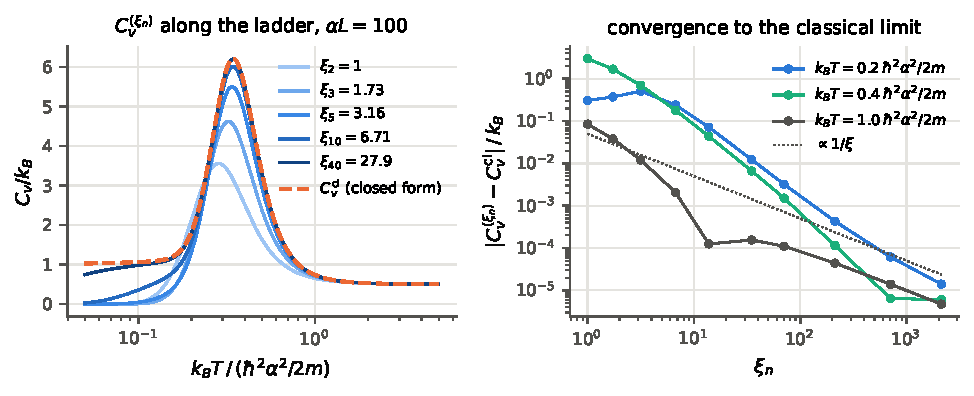
\includegraphics[width=\textwidth]{fig_xi_ladder.pdf}
\caption{Left: $C_v^{(\xi_n)}$ against $\kB T/(\hbar^2\alpha^2/2m)$ along the integer ladder (blue, light to dark with increasing $\xi_n$), approaching the closed-form $\Ccl$ of Eq.~\eqref{eq:Cclclosed} (orange, dashed), for $\alpha L=100$. Right: the distance to $\Ccl$ against $\xi_n$ at three temperatures, with a $1/\xi$ guide.}
\label{fig:ladder}
\end{figure}

% =====================================================================
\section{Results: \texorpdfstring{$\Cq$}{Cq} vs.\ \texorpdfstring{$\Ccl$}{Ccl}}
\label{sec:results}

\subsection{The anomaly}
Figure~\ref{fig:cv} and Table~\ref{tab:anomaly} compare $\Cq$ (exact levels, Eq.~\eqref{eq:Cqsum}) with $\Ccl$ (Eq.~\eqref{eq:Cclclosed}). For $\alpha L\ge100$ there is a window just below the quantum peak in which $\Cq>\Ccl$. The excess grows with $\alpha L$: $+0.34\,\kB$ at $\alpha L=100$, $+2.59\,\kB$ at $\alpha L=400$, and $+4.80\,\kB$ at $\alpha L=1000$. At $\alpha L=30$ the dimple produces no excess, and the only (tiny) positive difference is the wall term of Sec.~\ref{sec:walls}.

\begin{table}[h]
\centering
\caption{Quantum vs.\ classical heat capacity. All temperatures are $\kB T$ in units of $\hbar^2\alpha^2/2m$. ``Windows'' lists the temperature intervals where $\Cq-\Ccl>10^{-3}\kB$. The grid ends at $\kB T=5\,(\hbar^2\alpha^2/2m)$, so an upper edge of 5 is the end of the grid.}
\label{tab:anomaly}
\resizebox{\textwidth}{!}{%
\begin{tabular}{ccccccccc}
\toprule
$\alpha L$ & $\max(\Cq-\Ccl)/\kB$ & at $\kB T$ & $\Cq/\kB$ & $\Ccl/\kB$ & windows ($\kB T$) & $\Cq$ peak ($\kB T$) & $\Ccl$ peak ($\kB T$) & $\min(\Cq-\Ccl)/\kB$ ($\kB T$)\\
\midrule
30 & $+0.007$ & 3.668 & 0.524 & 0.517 & $[2.11,5]$ & 2.00 (0.392) & 3.74 (0.410) & $-1.75$ (0.419)\\
100 & $+0.343$ & 0.209 & 2.400 & 2.057 & $[0.177,0.238]$; $[2.69,5]$ & 3.56 (0.285) & 6.21 (0.344) & $-3.18$ (0.367)\\
400 & $+2.590$ & 0.183 & 5.048 & 2.458 & $[0.130,0.223]$ & 6.05 (0.216) & 10.02 (0.285) & $-6.20$ (0.298)\\
1000 & $+4.801$ & 0.167 & 7.446 & 2.645 & $[0.112,0.202]$ & 8.13 (0.185) & 13.13 (0.252) & $-9.10$ (0.263)\\
\bottomrule
\end{tabular}}
\end{table}

\begin{figure}[h]
\centering
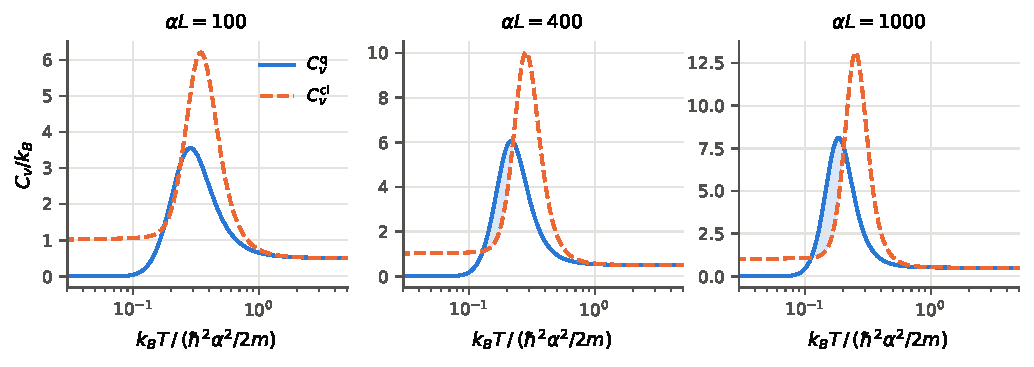
\includegraphics[width=\textwidth]{fig_cv_compare.pdf}
\caption{$\Cq$ (blue, solid) and $\Ccl$ (orange, dashed) against $\kB T/(\hbar^2\alpha^2/2m)$ for three box lengths. The shaded regions are where $\Cq>\Ccl$.}
\label{fig:cv}
\end{figure}

\subsection{Mechanism}
Both curves are dominated by one event: the particle leaving the well for the box (desorption). The difference lies in the binding.
\begin{itemize}[itemsep=2pt]
\item \textbf{Quantum.} The well holds a single state at $E_b=-\hbar^2\alpha^2/2m$, half the classical depth $\hbar^2\alpha^2/m$, because the zero-point energy is $\hbar^2\alpha^2/2m$. The bound ``phase'' has zero entropy and no internal heat capacity. Equal weights of the bound state and the box, $e^{\beta\hbar^2\alpha^2/2m}=L/\lth$, give the crossover temperature $T_q$ through
\begin{equation}
\frac{\hbar^2\alpha^2}{2m\kB T_q}=\ln\!\left(L\sqrt{\frac{m\kB T_q}{2\pi\hbar^2}}\right).
\end{equation}
\item \textbf{Classical.} The particle can sit at the floor $-\hbar^2\alpha^2/m$, but it pays a localization entropy: the well's weight is $e^{a}\sqrt{\pi/a}/\alpha$ with $a=\hbar^2\alpha^2/m\kB T$, from the harmonic bottom. Equating this to $L$ gives the crossover temperature $T_{\rm cl}$ through
\begin{equation}
a_{\rm cl}-\frac12\ln a_{\rm cl}=\ln\frac{\alpha L}{\sqrt\pi},\qquad a_{\rm cl}=\frac{\hbar^2\alpha^2}{m\kB T_{\rm cl}}.
\end{equation}
\end{itemize}
These rough equal-weight estimates give $(\kB T_q,\kB T_{\rm cl})=(0.354,0.415)$, $(0.248,0.315)$ and $(0.206,0.273)$, in units of $\hbar^2\alpha^2/2m$, for $\alpha L=100$, 400 and 1000. They run 10--25\% above the computed peak positions in Table~\ref{tab:anomaly}, but they reproduce the ordering $T_q<T_{\rm cl}$ and the growth of the shift with $\alpha L$.

The quantum peak therefore comes first. It is sharp because the quantum system jumps from a single state into a gas of $L/\lth$ states. The classical peak comes later and is taller. The anomaly window is the stretch where the quantum transition is under way and the classical one has not yet begun. Right after the window the order reverses, with a deficit reaching $\Cq-\Ccl=-9.10\,\kB$ at $\kB T=0.263\,(\hbar^2\alpha^2/2m)$ for $\alpha L=1000$ (last column of Table~\ref{tab:anomaly}). The anomaly is therefore a \emph{shift} of the peak to lower temperature, not a larger peak.

\subsection{The wall term}
\label{sec:walls}
At high $T$, the quantum interaction term $G\simeq2\sqrt{\beta\hbar^2\alpha^2/2\pi m}$ and the classical term $I/\lth\simeq2\sqrt{\beta\hbar^2\alpha^2/2\pi m}$ coincide. The difference between $\ln Z_q$ and $\ln Z_{\rm cl}$ is then dominated by the Dirichlet term: $\ln Z_q-\ln Z_{\rm cl}\simeq-\lth/(2L)\propto\beta^{1/2}$, which gives
\begin{equation}
\Cq-\Ccl\;\xrightarrow{T\to\infty}\;\kB\frac{\lth}{8L}>0 .
\end{equation}
This excess has nothing to do with the well. The empty box shows it too: its $\Cq$ peaks at $0.5625\,\kB$ at $T=2.86\,E_g$, where $E_g=\pi^2\hbar^2/2mL^2$, and stays above $\kB/2$ for all $T>1.26\,E_g$. At $T=100\,E_g$ the computed excess is $0.0140\,\kB$, against $\lth/8L=0.0141$. It accounts for the high-temperature windows at $\alpha L=30$ and $100$ in Table~\ref{tab:anomaly}. It is a property of hard walls, and it must be kept separate from the dimple effect when an excess is reported.

One consequence: because $U_q-U_{\rm cl}\simeq\kB T\,\lth/(4L)\propto\sqrt T$ grows without bound, the integral $\int_0^\infty(\Cq-\Ccl)\,\dd T$ diverges. The zero-point sum rule $\int_0^\infty(\Cq-\Ccl)\,\dd T=-E_{\rm ZPE}$, which holds for smooth confining potentials, does not apply with hard walls.

% =====================================================================
\section{Using the exact spectrum to verify the DVR}
\label{sec:dvr}
Table~\ref{tab:dvr} and Fig.~\ref{fig:dvr} compare the exact levels of Sec.~\ref{sec:levels} ($\alpha L=60$, 120 levels) with two DVRs:
\begin{enumerate}[itemsep=1pt]
\item the repo's Colbert--Miller sinc-DVR \cite{colbertmiller1992}, called directly (\texttt{colbert\_miller\_dvr\_1d}) on a grid whose edges sit one $\Delta x$ inside the walls;
\item the Colbert--Miller DVR for a finite interval (Appendix~\ref{app:sinedvr}), whose basis vanishes exactly at $\pm L/2$.
\end{enumerate}

\begin{table}[h]
\centering
\caption{$\max|E^{\rm DVR}-E^{\rm exact}|$ in units of $\hbar^2\alpha^2/2m$, for PT ($\lambda=2$) in a box, $\alpha L=60$.}
\label{tab:dvr}
\begin{tabular}{ccccc}
\toprule
$\alpha\Delta x$ & sinc-DVR: bound & sinc-DVR: levels 1--20 & sinc-DVR: levels 1--119 & box DVR: all 120\\
\midrule
0.2 & $3.6\times10^{-15}$ & $1.9\times10^{-3}$ & $6.4\times10^{-2}$ & $2.3\times10^{-12}$\\
0.1 & $3.8\times10^{-14}$ & $9.4\times10^{-4}$ & $3.2\times10^{-2}$ & $1.6\times10^{-13}$\\
0.05 & $1.2\times10^{-13}$ & $4.7\times10^{-4}$ & $1.6\times10^{-2}$ & $4.8\times10^{-13}$\\
0.025 & $7.2\times10^{-13}$ & $2.3\times10^{-4}$ & $7.9\times10^{-3}$ & $1.8\times10^{-12}$\\
\bottomrule
\end{tabular}
\end{table}

\begin{figure}[h]
\centering
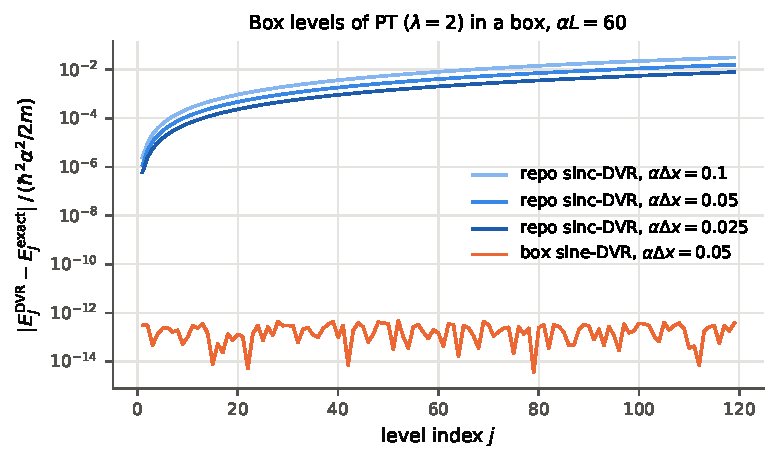
\includegraphics[width=0.75\textwidth]{fig_dvr_levels.pdf}
\caption{Error of each box level against the exact Eq.~\eqref{eq:quant}. The repo's sinc-DVR (blue) converges only linearly in $\Delta x$; the box DVR (orange) sits at round-off.}
\label{fig:dvr}
\end{figure}

Two conclusions follow.
\begin{enumerate}[itemsep=2pt]
\item \textbf{The repo's solver is correct for what it is built for.} The bound state lives far from the walls, and the sinc-DVR reproduces it to $10^{-13}\,(\hbar^2\alpha^2/2m)$ or better. The box levels converge only linearly: halving $\Delta x$ halves the error. That is not a solver bug. The sinc-DVR is built for the open line (as the project summaries note, it excludes hard walls), so the grid edges act as walls whose effective position is uncertain by a fraction of $\Delta x$. Since $E_j\propto1/L^2$, the error is $\delta E_j\approx2E_j\,\delta L/L$, which grows with $j$ exactly as in Fig.~\ref{fig:dvr}. It propagates into thermodynamics: at $\alpha L=60$, $\alpha\Delta x=0.05$ and $\kB T=2\,(\hbar^2\alpha^2/2m)$, the sinc-DVR spectrum gives $\ln Z_q=3.201010$, against the exact $3.201205$.
\item \textbf{A box mode needs the box DVR.} The finite-interval formula reproduces all 120 levels to $\le2.3\times10^{-12}\,(\hbar^2\alpha^2/2m)$, even at $\alpha\Delta x=0.2$. It would be the right engine if the pipeline is extended to hard-wall potentials. That is a change to \texttt{src/}, not made here.
\end{enumerate}

% =====================================================================
\section{Homogeneous (scale-invariant) strokes}
\label{sec:stroke}
Table~I of Ref.~\cite{deffner2014} lists the P\"oschl--Teller well and the infinite square well as two separate scale-invariant potentials. The system studied here is their sum. This section proves that the sum is again scale-invariant, and that this holds only when both components are driven with the same factor $\gamma$.

\subsection{Definition}
Deffner \emph{et al.} call a driving scale-invariant when the Hamiltonian keeps the form of their Eq.~(3). For a dilation about $x=0$ (their $f=0$; their $U$ and $q$ are our $V$ and $x$), this form is
\begin{equation}
H(\gamma)=\frac{p^2}{2m}+\frac{1}{\gamma^2}\,V_0\!\left(\frac{x}{\gamma}\right),\qquad V_0(x)=V(x)\big|_{\gamma=1}.
\label{eq:Hscale}
\end{equation}
A family of potentials $V(x;\mu)$, with control parameters $\mu$, therefore admits a scale-invariant stroke if there is a path $\mu(\gamma)$, $\gamma>0$, with $\mu(1)=\mu_0$ and
\begin{equation}
V\big(x;\mu(\gamma)\big)=\frac{1}{\gamma^2}\,V\!\left(\frac{x}{\gamma};\mu_0\right)\qquad\text{for all }x\in\mathbb R\text{ and all }\gamma>0 .
\label{eq:scaleinv}
\end{equation}
The shape of the potential is then fixed: only its length scale (times $\gamma$) and its energy scale (times $\gamma^{-2}$) change. Write $\mathcal S_\gamma$ for the map that takes a potential $U(x)$ to
\begin{equation}
(\mathcal S_\gamma U)(x)\equiv\frac{1}{\gamma^2}\,U\!\left(\frac{x}{\gamma}\right),
\label{eq:Sgamma}
\end{equation}
so that Eq.~\eqref{eq:scaleinv} reads $V(\cdot\,;\mu(\gamma))=\mathcal S_\gamma V(\cdot\,;\mu_0)$. Two properties of $\mathcal S_\gamma$ are used below.
\begin{enumerate}[label=(\roman*),itemsep=2pt]
\item \emph{Linearity.} $\mathcal S_\gamma(U_1+U_2)=\mathcal S_\gamma U_1+\mathcal S_\gamma U_2$, because the same argument $x/\gamma$ is inserted in both terms and both are multiplied by the same factor $\gamma^{-2}$.
\item \emph{Hard walls.} $\mathcal S_\gamma$ maps $+\infty$ to $+\infty$, because $0<\gamma^{-2}<\infty$. With the convention (finite)$\,+\,\infty=+\infty$, property (i) also holds at points where one of the terms is infinite.
\end{enumerate}

\subsection{Each component is scale-invariant}
Write Eq.~\eqref{eq:Vgeneral} as the sum of its two components,
\begin{equation}
V(x;\alpha,L)=V_{\rm PT}(x;\alpha)+V_{\rm box}(x;L),
\label{eq:Vsplit}
\end{equation}
\[
V_{\rm PT}(x;\alpha)=-\frac{\hbar^2}{2m}\,\alpha^2\,\frac{\lambda(\lambda-1)}{\cosh^2(\alpha x)}\quad(x\in\mathbb R),\qquad
V_{\rm box}(x;L)=\begin{cases}0,&|x|<L/2,\\+\infty,&|x|\ge L/2.\end{cases}
\]
Inside the box the sum equals $V_{\rm PT}$, and outside it is $+\infty$, which is Eq.~\eqref{eq:Vgeneral}. Both components are centred at $x=0$, the centre of the dilation.

\paragraph{P\"oschl--Teller well.} Table~I drives the well with $\alpha\to\alpha/\gamma$ at fixed $\lambda$. Then
\begin{align}
V_{\rm PT}\!\left(x;\frac{\alpha}{\gamma}\right)&=-\frac{\hbar^2}{2m}\,\frac{\alpha^2}{\gamma^2}\,\frac{\lambda(\lambda-1)}{\cosh^2(\alpha x/\gamma)}\nonumber\\
&=\frac{1}{\gamma^2}\left[-\frac{\hbar^2}{2m}\,\alpha^2\,\frac{\lambda(\lambda-1)}{\cosh^2\!\big(\alpha\cdot(x/\gamma)\big)}\right]=\frac{1}{\gamma^2}\,V_{\rm PT}\!\left(\frac{x}{\gamma};\alpha\right),
\label{eq:PTscale}
\end{align}
which is Eq.~\eqref{eq:scaleinv} with $\mu=\alpha$. The factor $\alpha^2$ in front supplies the $\gamma^{-2}$, and the $\alpha$ inside the $\cosh$ supplies the argument $x/\gamma$. The parameter $\lambda$ must stay fixed, because it sets the depth in units of $\hbar^2\alpha^2/2m$, i.e.\ the shape.

\paragraph{Box.} The box is driven with $L\to\gamma L$. Since $|x|<\gamma L/2\iff|x/\gamma|<L/2$,
\begin{equation}
V_{\rm box}(x;\gamma L)=\begin{cases}0,&|x/\gamma|<L/2,\\+\infty,&|x/\gamma|\ge L/2,\end{cases}
\qquad
\frac{1}{\gamma^2}\,V_{\rm box}\!\left(\frac{x}{\gamma};L\right)=\begin{cases}\gamma^{-2}\cdot0=0,&|x/\gamma|<L/2,\\\gamma^{-2}\cdot\infty=+\infty,&|x/\gamma|\ge L/2.\end{cases}
\label{eq:boxscale}
\end{equation}
The two sides agree for every $x$, so the box satisfies Eq.~\eqref{eq:scaleinv} with $\mu=L$. This is the $b\to\infty$ limit of Table~I's power-law row, $A|x|^b$ with $A\to A/\gamma^{2+b}$: writing $A=E_0(2/L)^b$ at fixed $E_0>0$, so that $A|x|^b=E_0(2|x|/L)^b$ tends to $V_{\rm box}$, the rule becomes $L\to\gamma^{1+2/b}L$, which tends to $L\to\gamma L$.

\subsection{The sum is scale-invariant}
\paragraph{Proposition.} Drive both components with the same $\gamma$: $\alpha\to\alpha/\gamma$ and $L\to\gamma L$, with $\lambda$ fixed. Then the potential of Eq.~\eqref{eq:Vsplit} satisfies Eq.~\eqref{eq:scaleinv},
\begin{equation}
V\!\left(x;\frac{\alpha}{\gamma},\gamma L\right)=\frac{1}{\gamma^2}\,V\!\left(\frac{x}{\gamma};\alpha,L\right)\qquad\text{for all }x\in\mathbb R\text{ and all }\gamma>0 .
\label{eq:sumscale}
\end{equation}

\paragraph{Proof.} By Eqs.~\eqref{eq:PTscale} and \eqref{eq:boxscale}, and then linearity (i),
\[
V\!\left(x;\frac{\alpha}{\gamma},\gamma L\right)=V_{\rm PT}\!\left(x;\frac{\alpha}{\gamma}\right)+V_{\rm box}(x;\gamma L)
=\frac{1}{\gamma^2}V_{\rm PT}\!\left(\frac x\gamma;\alpha\right)+\frac{1}{\gamma^2}V_{\rm box}\!\left(\frac x\gamma;L\right)
=\frac{1}{\gamma^2}\,V\!\left(\frac{x}{\gamma};\alpha,L\right).
\]
Inside the moved walls, $|x|<\gamma L/2$, every term is finite and this is ordinary algebra. Outside, both sides are $+\infty$ by property (ii). $\square$

\medskip
The composite potential is therefore of the form of Eq.~(3) of Ref.~\cite{deffner2014}, with $V_0(x)=V(x;\alpha,L)$, the well in its box at $\gamma=1$. Every result derived there for an arbitrary $V_0$ applies to it unchanged, including the first row of their Table~I.

\paragraph{The common $\gamma$ is necessary.} Suppose instead that the components are driven with different factors, $\alpha\to\alpha/\gamma_1$ and $L\to\gamma_2L$ with $\gamma_1\neq\gamma_2$, and that the result still had the form $c^{-2}V(x/c;\alpha,L)$ for some $c>0$.
\begin{itemize}[itemsep=2pt]
\item The walls of $c^{-2}V(x/c;\alpha,L)$ are at $\pm cL/2$, and those of the driven potential are at $\pm\gamma_2L/2$. Hence $c=\gamma_2$.
\item At $x=0$ the two sides take the values
\[
V\!\left(0;\frac{\alpha}{\gamma_1},\gamma_2L\right)=-\frac{\hbar^2}{2m}\,\frac{\alpha^2}{\gamma_1^2}\,\lambda(\lambda-1),\qquad
\frac{1}{\gamma_2^2}\,V(0;\alpha,L)=-\frac{\hbar^2}{2m}\,\frac{\alpha^2}{\gamma_2^2}\,\lambda(\lambda-1).
\]
These agree only if $\gamma_1=\gamma_2$, a contradiction.
\end{itemize}
Each component is still a member of its own Table~I family, but the sum is not scale-invariant: its shape has changed. The shape of Eq.~\eqref{eq:Vgeneral} is fixed by its two dimensionless parameters, $\lambda$ and the ratio $\alpha L$ of box length to well width. A scale-invariant stroke must keep both fixed, and $\alpha\to\alpha/\gamma$, $L\to\gamma L$ is the only such stroke that changes the scale. If the well were centred at some $x_0\neq0$, the same argument would require $x_0\to\gamma x_0$ as well.

\subsection{Consequences}
\paragraph{Levels and eigenfunctions.} Let $\psi_n$ solve the $\gamma=1$ problem, $-\frac{\hbar^2}{2m}\psi_n''+V(x;\alpha,L)\,\psi_n=E_n\psi_n$ with $\psi_n(\pm L/2)=0$, and define $\psi_n^{(\gamma)}(x)=\gamma^{-1/2}\psi_n(x/\gamma)$, the eigenfunction map of Ref.~\cite{deffner2014} (their Appendix~A). Using $\mathrm{d}^2\psi_n(x/\gamma)/\mathrm{d}x^2=\gamma^{-2}\psi_n''(x/\gamma)$ for the kinetic term and Eq.~\eqref{eq:sumscale} for the potential,
\[
-\frac{\hbar^2}{2m}\dv[2]{\psi_n^{(\gamma)}}{x}+V\!\left(x;\frac\alpha\gamma,\gamma L\right)\psi_n^{(\gamma)}
=\frac{\gamma^{-1/2}}{\gamma^2}\left[-\frac{\hbar^2}{2m}\psi_n''+V(\,\cdot\,;\alpha,L)\,\psi_n\right]\!\left(\frac x\gamma\right)=\frac{E_n}{\gamma^2}\,\psi_n^{(\gamma)}(x).
\]
The boundary condition moves with the walls, $\psi_n^{(\gamma)}(\pm\gamma L/2)=\gamma^{-1/2}\psi_n(\pm L/2)=0$, and the norm is kept, $\int|\psi_n^{(\gamma)}(x)|^2\dd x=\int|\psi_n(y)|^2\dd y$ with $x=\gamma y$. The map $\psi\mapsto\gamma^{-1/2}\psi(x/\gamma)$ is invertible, so every eigenstate of the driven problem arises in this way. Hence, for every $n$,
\begin{equation}
E_n\!\left(\frac\alpha\gamma,\gamma L\right)=\frac{1}{\gamma^2}\,E_n(\alpha,L).
\label{eq:Escale}
\end{equation}
This uses only Eq.~\eqref{eq:sumscale}, not the exact solution of Sec.~\ref{sec:levels}. The exact solution confirms it: under $\alpha\to\alpha/\gamma$, $L\to\gamma L$, the product $\alpha L$ is unchanged and $\alpha\tanh(\alpha L/2)\to\alpha\tanh(\alpha L/2)/\gamma$, so the roots of Eqs.~\eqref{eq:quant}--\eqref{eq:bound} scale as $k_j\to k_j/\gamma$ and $\kappa_b\to\kappa_b/\gamma$.

\paragraph{Partition functions and heat capacities.} By Eq.~\eqref{eq:Escale},
\[
Z_q\!\left(\beta;\frac\alpha\gamma,\gamma L\right)=\sum_ne^{-\beta E_n(\alpha,L)/\gamma^2}=Z_q\!\left(\frac{\beta}{\gamma^2};\alpha,L\right).
\]
Classically, substituting $x=\gamma y$ in Eq.~\eqref{eq:Zcl} and using Eq.~\eqref{eq:sumscale},
\[
Z_{\rm cl}\!\left(\beta;\frac\alpha\gamma,\gamma L\right)=\frac{1}{\lth(\beta)}\int e^{-\beta V(x;\alpha/\gamma,\gamma L)}\dd x=\frac{\gamma}{\lth(\beta)}\int e^{-(\beta/\gamma^2)V(y;\alpha,L)}\dd y=Z_{\rm cl}\!\left(\frac{\beta}{\gamma^2};\alpha,L\right),
\]
because $\lth\propto\beta^{1/2}$ gives $\gamma/\lth(\beta)=1/\lth(\beta/\gamma^2)$. In both cases the stroke only rescales $\beta\to\beta/\gamma^2$. With $\beta'=\beta/\gamma^2$ one has $\beta^2\partial_\beta^2=\beta'^2\partial_{\beta'}^2$, so $C_v=\kB\beta^2\partial_\beta^2\ln Z$ gives
\begin{equation}
C_v(T;\gamma)=C_v(\gamma^2T;1)\qquad\text{for both }\Cq\text{ and }\Ccl .
\label{eq:Cvscale}
\end{equation}
This agrees with Sec.~\ref{sec:model}: $C_v$ depends only on $\alpha L$, which the stroke keeps, and on $2m\kB T/\hbar^2\alpha^2$, which is the same at $(T,\alpha/\gamma)$ as at $(\gamma^2T,\alpha)$. The stroke therefore preserves the shape of $C_v(T)$ and moves every feature at a temperature $T^*$ to $T^*/\gamma^2$, including the anomaly window of Sec.~\ref{sec:results}. An expansion ($\gamma>1$) moves the window to lower temperature, and a compression ($\gamma<1$) moves it up.

\paragraph{The stroke is not the $\xi$ formula.} The two must not be confused. The stroke keeps $\lambda$, and hence the reflectionless structure, fixed. The $\xi$ formula changes $\lambda$ through Eq.~\eqref{eq:lamxi}, because it holds the well depth $\frac{\hbar^2\alpha^2}{2m}\lambda(\lambda-1)$ fixed while $\hbar\to\hbar/\xi$, so $\lambda(\lambda-1)$ must grow as $\xi^2$.

% =====================================================================
\section{Summary and reproduction}
\begin{itemize}[itemsep=2pt]
\item The spectrum of a reflectionless P\"oschl--Teller well in a box is given exactly by Eqs.~\eqref{eq:quant} and \eqref{eq:bound}, at any $L$, and $Z_q$ has the closed form of Eq.~\eqref{eq:Zqclosed}.
\item $\Cq$ follows from the variance formula, Eq.~\eqref{eq:var}, either by direct summation or in closed form via Eq.~\eqref{eq:Cqclosed}; the two agree to $10^{-12}\kB$.
\item The $\xi$ formula is evaluated exactly along the ladder $\xi_n=\sqrt{n(n-1)/2}$. Its limit is taken analytically and equals the classical phase-space result, Eq.~\eqref{eq:Cclclosed}.
\item $\Cq>\Ccl$ in a window just below the quantum desorption peak, by up to $+4.8\,\kB$ at $\alpha L=1000$. A separate, small excess $\lth/(8L)$ at high $T$ comes from the walls alone.
\item The exact spectrum shows that the repo's sinc-DVR handles the bound state exactly but represents hard walls only to $\mathcal O(\Delta x)$, while a box DVR is exact.
\item The sum of the two scale-invariant potentials of Table~I in Ref.~\cite{deffner2014}, the P\"oschl--Teller well and the box, is itself scale-invariant, Eq.~\eqref{eq:sumscale}, provided both are driven with the same $\gamma$ (fixed $\alpha L$). Every level then scales as $E_n\to E_n/\gamma^2$, and $C_v(T;\gamma)=C_v(\gamma^2T;1)$.
\end{itemize}
\noindent\textbf{Reproduction.} From the repository root:
\begin{center}
\texttt{python verification/pt\_box/pt\_box\_check.py}
\end{center}
The script runs in about 20~s on either of the project's Python environments. It rewrites \texttt{RESULTS.md} and \texttt{figures/}, from which every table and figure above is taken.

% =====================================================================
\appendix
\section{Direct check of the solution \texorpdfstring{$\psi_k$}{psi\_k}}
\label{app:check}
With $u=\tanh(\alpha x)$ and $u'=\alpha(1-u^2)$,
\begin{align*}
\psi_k&=(\alpha u-ik)e^{ikx},\\
\psi_k'&=\big[\alpha^2(1-u^2)+ik\alpha u+k^2\big]e^{ikx},\\
\psi_k''&=\big[-2\alpha^3u(1-u^2)+2ik\alpha^2(1-u^2)-k^2\alpha u+ik^3\big]e^{ikx}.
\end{align*}
The Schr\"odinger equation $-\frac{\hbar^2}{2m}\psi''+V\psi=E\psi$ is $-\psi''-2\alpha^2(1-u^2)\psi=k^2\psi$, since $\frac{2m}{\hbar^2}V=-2\alpha^2/\cosh^2(\alpha x)=-2\alpha^2(1-u^2)$ and $E=\hbar^2k^2/2m$. Substituting,
\[
-\psi_k''-2\alpha^2(1-u^2)\psi_k=\big[k^2\alpha u-ik^3\big]e^{ikx}=k^2(\alpha u-ik)e^{ikx}=k^2\psi_k .\qquad\checkmark
\]

\section{A Gaussian--Lorentzian integral}
\label{app:gaussint}
For any constant $c>0$ (Sec.~\ref{sec:Zclosed} uses $c=\alpha\tanh(\alpha L/2)$), let $\mathcal F(b)=\int_0^\infty e^{-bk^2}/(k^2+c^2)\,\dd k$. Then
\[
\mathcal F'(b)-c^2\mathcal F(b)=-\int_0^\infty e^{-bk^2}\dd k=-\frac12\sqrt{\frac{\pi}{b}},
\qquad\text{so}\qquad
\dv{b}\big(e^{-bc^2}\mathcal F\big)=-\frac12\sqrt{\frac\pi b}\,e^{-bc^2}.
\]
Integrating from $b$ to $\infty$, where $e^{-bc^2}\mathcal F\to0$, and substituting $s=u^2/c^2$,
\[
\mathcal F(b)=e^{bc^2}\int_b^\infty\frac12\sqrt{\frac\pi s}\,e^{-sc^2}\dd s=\frac{\sqrt\pi}{c}\,e^{bc^2}\int_{c\sqrt b}^\infty e^{-u^2}\dd u=\frac{\pi}{2c}\,e^{bc^2}\erfc\!\left(c\sqrt b\right).
\]

\section{The classical well integrals}
\label{app:classint}
With $t=\tanh(\alpha x)$ we have $\dd x/\cosh^2(\alpha x)=\dd t/\alpha$ and $1/\cosh^2(\alpha x)=1-t^2$, so
\begin{align*}
\alpha J_1(a)&=\int_{-1}^1e^{a(1-t^2)}\dd t=2e^a\int_0^1e^{-at^2}\dd t=\sqrt\pi\,\frac{e^a\erf\sqrt a}{\sqrt a},\\
\alpha J_2(a)&=\int_{-1}^1(1-t^2)\,e^{a(1-t^2)}\dd t=\alpha J_1'(a).
\end{align*}
Differentiating, and using $\mathrm{d}\erf\sqrt a/\mathrm{d}a=e^{-a}/\sqrt{\pi a}$,
\[
\alpha J_1'(a)=\sqrt\pi\,e^a\erf\sqrt a\left(a^{-1/2}-\tfrac12a^{-3/2}\right)+\frac1a=\alpha J_1(a)\left(1-\frac1{2a}\right)+\frac1a .
\]
Also $\dd(\alpha I)/\dd a=\alpha J_1$, consistent with Eq.~\eqref{eq:Iseries}.

\section{The box (finite-interval) DVR}
\label{app:sinedvr}
For the interval $(-L/2,L/2)$ with $N-1$ interior points $x_i=-L/2+iL/N$, the Colbert--Miller kinetic matrix \cite{colbertmiller1992} is
\begin{align*}
T_{ii}&=\frac{\hbar^2}{2m}\,\frac{\pi^2}{2L^2}\left[\frac{2N^2+1}{3}-\frac{1}{\sin^2(\pi i/N)}\right],\\
T_{ij}&=\frac{\hbar^2}{2m}\,\frac{\pi^2}{2L^2}\,(-1)^{i-j}\left[\frac{1}{\sin^2\!\big(\pi(i-j)/2N\big)}-\frac{1}{\sin^2\!\big(\pi(i+j)/2N\big)}\right]\quad(i\neq j).
\end{align*}
Its basis functions vanish at $x=\pm L/2$, so the hard walls are imposed exactly. With $V_{ij}=V(x_i)\delta_{ij}$, the free-box levels are reproduced exactly up to the grid's highest mode.

% =====================================================================
\begin{thebibliography}{9}

\bibitem{gelbwaser2018}
D. Gelbwaser-Klimovsky, A. Bylinskii, D. Gangloff, R. Islam, A. Aspuru-Guzik, and V. Vuleti\'c, ``Single-atom heat machines enabled by energy quantization,'' \emph{Phys. Rev. Lett.} \textbf{120}, 170601 (2018).

\bibitem{deffner2014}
S. Deffner, C. Jarzynski, and A. del Campo, ``Classical and quantum shortcuts to adiabaticity for scale-invariant driving,'' \emph{Phys. Rev. X} \textbf{4}, 021013 (2014).

\bibitem{flugge1971}
S. Fl\"ugge, \emph{Practical Quantum Mechanics}, Vol.~I (Springer, Heidelberg, 1971).

\bibitem{poschlteller1933}
G. P\"oschl and E. Teller, ``Bemerkungen zur Quantenmechanik des anharmonischen Oszillators,'' \emph{Z. Phys.} \textbf{83}, 143 (1933).

\bibitem{cooper1995}
F. Cooper, A. Khare, and U. Sukhatme, ``Supersymmetry and quantum mechanics,'' \emph{Phys. Rep.} \textbf{251}, 267 (1995).

\bibitem{bethuhlenbeck1937}
E. Beth and G. E. Uhlenbeck, ``The quantum theory of the non-ideal gas. II. Behaviour at low temperatures,'' \emph{Physica} \textbf{4}, 915 (1937).

\bibitem{colbertmiller1992}
D. T. Colbert and W. H. Miller, ``A novel discrete variable representation for quantum mechanical reactive scattering via the S-matrix Kohn method,'' \emph{J. Chem. Phys.} \textbf{96}, 1982 (1992).

\end{thebibliography}

\end{document}
